% === Begin Label Data ===
% ID: 455
% 难度星级: 
% 标签: 
% 备注: 
% 组卷引用次数: 0
% === End  Label Data ===

\begin{problem}{2015}{G}{浙江卷（文）}{7}{圆锥曲线}
如图，斜线段 $ AB $ 与平面 $ \alpha $ 所成的角为 $ 60^\circ $，$ B $ 为斜足，平面 $ \alpha $ 上的动点 $ P $ 满足 $ \angle PAB = 30^\circ $，则点 $ P $ 的轨迹是 （\hspace{1cm}）
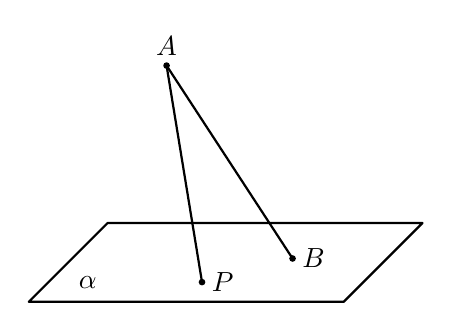
\begin{tikzpicture}[scale=1.0,line cap=round,line join=round]
\usetikzlibrary{calc}

% plane alpha as a parallelogram
\coordinate (L1) at (-2,0);
\coordinate (L2) at ( 2,0);
\coordinate (L3) at ( 3,1.0);
\coordinate (L4) at (-1,1.0);
\draw[thick] (L1)--(L2)--(L3)--(L4)--cycle;
\node at (-1.25,0.25) {$\alpha$};

% points on the plane
\coordinate (P) at (0.2,0.25);
\coordinate (B) at (1.35,0.55);
\fill (P) circle (1.2pt) node[right] {$P$};
\fill (B) circle (1.2pt) node[right] {$B$};

% point A above the plane
\coordinate (A) at (-0.25,3.0);
\fill (A) circle (1.2pt) node[above] {$A$};

% segments
\draw[thick] (A)--(B);
\draw[thick] (A)--(P);

\end{tikzpicture}
\begin{choices}
\choice{{直线}}
\choice{{抛物线}}
\choice{{椭圆}}
\choice{{双曲线的一支}}
\end{choices}

\end{problem}